% Short (5-page) version of main.tex for ICIIT 2027 (ACM proceedings, 4-5 two-column pages).
% Same numbers and protocol as main.tex; the follow-up experiments are summarised briefly
% and reported in full in main.tex and ../PROTOCOL.md.
\documentclass[sigconf]{acmart}

\usepackage{booktabs}
\usepackage{graphicx}
\usepackage{microtype}
\usepackage{amsmath}

% Generated by scripts/07_paper_assets.py from results files. Do not edit by hand.
\makeatletter
\newcommand{\res}[1]{\@ifundefined{res@#1}{\textbf{??#1??}}{\csname res@#1\endcsname}}
\expandafter\def\csname res@binding-rho0.3\endcsname{94.3}
\expandafter\def\csname res@binding-rho0.5\endcsname{86.5}
\expandafter\def\csname res@binding-rho0.7\endcsname{70.8}
\expandafter\def\csname res@cmp-nn-baselines-pmax\endcsname{0.00052}
\expandafter\def\csname res@cmp-nn-baselines-sig\endcsname{12}
\expandafter\def\csname res@cmp-nn-baselines-total\endcsname{12}
\expandafter\def\csname res@cmp-nn-lgb-pmax\endcsname{0.0026}
\expandafter\def\csname res@cmp-nn-lgb-sig\endcsname{6}
\expandafter\def\csname res@cmp-nn-lgb-total\endcsname{6}
\expandafter\def\csname res@cmp-q09-baselines-pmax\endcsname{6.7e-49}
\expandafter\def\csname res@cmp-q09-baselines-sig\endcsname{24}
\expandafter\def\csname res@cmp-q09-baselines-total\endcsname{24}
\expandafter\def\csname res@cmp-tft-nhits-pmax\endcsname{1}
\expandafter\def\csname res@cmp-tft-nhits-sig\endcsname{1}
\expandafter\def\csname res@cmp-tft-nhits-total\endcsname{3}
\expandafter\def\csname res@data-campaigns\endcsname{414}
\expandafter\def\csname res@data-campaigns-total\endcsname{675}
\expandafter\def\csname res@data-eval-impressions\endcsname{4{,}197{,}856}
\expandafter\def\csname res@data-impressions\endcsname{16{,}468{,}027}
\expandafter\def\csname res@data-spend-share\endcsname{91.7}
\expandafter\def\csname res@data-test-episodes\endcsname{2{,}070}
\expandafter\def\csname res@even-rho0.3-bur\endcsname{93.8}
\expandafter\def\csname res@even-rho0.3-click\endcsname{0.993}
\expandafter\def\csname res@even-rho0.3-click-hi\endcsname{1.000}
\expandafter\def\csname res@even-rho0.3-click-lo\endcsname{0.987}
\expandafter\def\csname res@even-rho0.3-conv\endcsname{0.997}
\expandafter\def\csname res@even-rho0.3-early\endcsname{15.0}
\expandafter\def\csname res@even-rho0.3-pvi\endcsname{0.342}
\expandafter\def\csname res@even-rho0.5-bur\endcsname{90.2}
\expandafter\def\csname res@even-rho0.5-click\endcsname{0.960}
\expandafter\def\csname res@even-rho0.5-click-hi\endcsname{0.967}
\expandafter\def\csname res@even-rho0.5-click-lo\endcsname{0.954}
\expandafter\def\csname res@even-rho0.5-conv\endcsname{0.966}
\expandafter\def\csname res@even-rho0.5-early\endcsname{6.4}
\expandafter\def\csname res@even-rho0.5-pvi\endcsname{0.314}
\expandafter\def\csname res@even-rho0.7-bur\endcsname{84.8}
\expandafter\def\csname res@even-rho0.7-click\endcsname{0.942}
\expandafter\def\csname res@even-rho0.7-click-hi\endcsname{0.950}
\expandafter\def\csname res@even-rho0.7-click-lo\endcsname{0.935}
\expandafter\def\csname res@even-rho0.7-conv\endcsname{0.946}
\expandafter\def\csname res@even-rho0.7-early\endcsname{2.8}
\expandafter\def\csname res@even-rho0.7-pvi\endcsname{0.261}
\expandafter\def\csname res@fc-early-max\endcsname{6.1}
\expandafter\def\csname res@fc-early-min\endcsname{3.4}
\expandafter\def\csname res@fc-lightgbm-cov80\endcsname{71.7}
\expandafter\def\csname res@fc-lightgbm-cross\endcsname{0.92}
\expandafter\def\csname res@fc-lightgbm-mase\endcsname{0.853}
\expandafter\def\csname res@fc-lightgbm-mase-sd\endcsname{0.000}
\expandafter\def\csname res@fc-lightgbm-mase-step1\endcsname{0.810}
\expandafter\def\csname res@fc-lightgbm-mase-step24\endcsname{0.871}
\expandafter\def\csname res@fc-lightgbm-medmase\endcsname{0.722}
\expandafter\def\csname res@fc-lightgbm-spl0.1\endcsname{0.080}
\expandafter\def\csname res@fc-lightgbm-spl0.5\endcsname{0.246}
\expandafter\def\csname res@fc-lightgbm-spl0.9\endcsname{0.185}
\expandafter\def\csname res@fc-naive-cov80\endcsname{60.6}
\expandafter\def\csname res@fc-naive-cross\endcsname{0.00}
\expandafter\def\csname res@fc-naive-mase\endcsname{0.917}
\expandafter\def\csname res@fc-naive-mase-sd\endcsname{0.000}
\expandafter\def\csname res@fc-naive-mase-step1\endcsname{0.920}
\expandafter\def\csname res@fc-naive-mase-step24\endcsname{0.908}
\expandafter\def\csname res@fc-naive-medmase\endcsname{0.793}
\expandafter\def\csname res@fc-naive-spl0.1\endcsname{0.095}
\expandafter\def\csname res@fc-naive-spl0.5\endcsname{0.262}
\expandafter\def\csname res@fc-naive-spl0.9\endcsname{0.194}
\expandafter\def\csname res@fc-nhits-cov80\endcsname{75.8}
\expandafter\def\csname res@fc-nhits-cross\endcsname{0.47}
\expandafter\def\csname res@fc-nhits-mase\endcsname{0.794}
\expandafter\def\csname res@fc-nhits-mase-sd\endcsname{0.014}
\expandafter\def\csname res@fc-nhits-mase-step1\endcsname{0.719}
\expandafter\def\csname res@fc-nhits-mase-step24\endcsname{0.813}
\expandafter\def\csname res@fc-nhits-medmase\endcsname{0.723}
\expandafter\def\csname res@fc-nhits-spl0.1\endcsname{0.078}
\expandafter\def\csname res@fc-nhits-spl0.5\endcsname{0.231}
\expandafter\def\csname res@fc-nhits-spl0.9\endcsname{0.158}
\expandafter\def\csname res@fc-pvi-max\endcsname{0.12}
\expandafter\def\csname res@fc-pvi-min\endcsname{0.08}
\expandafter\def\csname res@fc-tft-cov80\endcsname{76.9}
\expandafter\def\csname res@fc-tft-cross\endcsname{0.03}
\expandafter\def\csname res@fc-tft-mase\endcsname{0.787}
\expandafter\def\csname res@fc-tft-mase-sd\endcsname{0.004}
\expandafter\def\csname res@fc-tft-mase-step1\endcsname{0.729}
\expandafter\def\csname res@fc-tft-mase-step24\endcsname{0.814}
\expandafter\def\csname res@fc-tft-medmase\endcsname{0.708}
\expandafter\def\csname res@fc-tft-spl0.1\endcsname{0.076}
\expandafter\def\csname res@fc-tft-spl0.5\endcsname{0.229}
\expandafter\def\csname res@fc-tft-spl0.9\endcsname{0.161}
\expandafter\def\csname res@gain-even-max\endcsname{5.4}
\expandafter\def\csname res@gain-even-min\endcsname{3.4}
\expandafter\def\csname res@gain-pid-max\endcsname{2.0}
\expandafter\def\csname res@gain-pid-min\endcsname{0.7}
\expandafter\def\csname res@hedge-bur-max\endcsname{82.8}
\expandafter\def\csname res@hedge-bur-min\endcsname{75.2}
\expandafter\def\csname res@hedge-cost-max\endcsname{10.6}
\expandafter\def\csname res@hedge-cost-min\endcsname{7.7}
\expandafter\def\csname res@hedge-early-max\endcsname{0.7}
\expandafter\def\csname res@hedge-early-min\endcsname{0.1}
\expandafter\def\csname res@hindsight-rho0.3-bur\endcsname{90.4}
\expandafter\def\csname res@hindsight-rho0.3-click\endcsname{1.000}
\expandafter\def\csname res@hindsight-rho0.3-click-hi\endcsname{1.000}
\expandafter\def\csname res@hindsight-rho0.3-click-lo\endcsname{1.000}
\expandafter\def\csname res@hindsight-rho0.3-conv\endcsname{1.000}
\expandafter\def\csname res@hindsight-rho0.3-early\endcsname{13.4}
\expandafter\def\csname res@hindsight-rho0.3-pvi\endcsname{0.000}
\expandafter\def\csname res@hindsight-rho0.5-bur\endcsname{90.6}
\expandafter\def\csname res@hindsight-rho0.5-click\endcsname{1.000}
\expandafter\def\csname res@hindsight-rho0.5-click-hi\endcsname{1.000}
\expandafter\def\csname res@hindsight-rho0.5-click-lo\endcsname{1.000}
\expandafter\def\csname res@hindsight-rho0.5-conv\endcsname{1.000}
\expandafter\def\csname res@hindsight-rho0.5-early\endcsname{9.5}
\expandafter\def\csname res@hindsight-rho0.5-pvi\endcsname{0.000}
\expandafter\def\csname res@hindsight-rho0.7-bur\endcsname{87.8}
\expandafter\def\csname res@hindsight-rho0.7-click\endcsname{1.000}
\expandafter\def\csname res@hindsight-rho0.7-click-hi\endcsname{1.000}
\expandafter\def\csname res@hindsight-rho0.7-click-lo\endcsname{1.000}
\expandafter\def\csname res@hindsight-rho0.7-conv\endcsname{1.000}
\expandafter\def\csname res@hindsight-rho0.7-early\endcsname{6.0}
\expandafter\def\csname res@hindsight-rho0.7-pvi\endcsname{0.000}
\expandafter\def\csname res@lightgbm-q0.5-rho0.3-bur\endcsname{94.6}
\expandafter\def\csname res@lightgbm-q0.5-rho0.3-click\endcsname{1.019}
\expandafter\def\csname res@lightgbm-q0.5-rho0.3-click-hi\endcsname{1.024}
\expandafter\def\csname res@lightgbm-q0.5-rho0.3-click-lo\endcsname{1.013}
\expandafter\def\csname res@lightgbm-q0.5-rho0.3-conv\endcsname{1.013}
\expandafter\def\csname res@lightgbm-q0.5-rho0.3-early\endcsname{5.6}
\expandafter\def\csname res@lightgbm-q0.5-rho0.3-pvi\endcsname{0.094}
\expandafter\def\csname res@lightgbm-q0.5-rho0.5-bur\endcsname{92.4}
\expandafter\def\csname res@lightgbm-q0.5-rho0.5-click\endcsname{0.997}
\expandafter\def\csname res@lightgbm-q0.5-rho0.5-click-hi\endcsname{1.003}
\expandafter\def\csname res@lightgbm-q0.5-rho0.5-click-lo\endcsname{0.989}
\expandafter\def\csname res@lightgbm-q0.5-rho0.5-conv\endcsname{0.998}
\expandafter\def\csname res@lightgbm-q0.5-rho0.5-early\endcsname{5.0}
\expandafter\def\csname res@lightgbm-q0.5-rho0.5-pvi\endcsname{0.094}
\expandafter\def\csname res@lightgbm-q0.5-rho0.7-bur\endcsname{88.5}
\expandafter\def\csname res@lightgbm-q0.5-rho0.7-click\endcsname{0.992}
\expandafter\def\csname res@lightgbm-q0.5-rho0.7-click-hi\endcsname{0.995}
\expandafter\def\csname res@lightgbm-q0.5-rho0.7-click-lo\endcsname{0.989}
\expandafter\def\csname res@lightgbm-q0.5-rho0.7-conv\endcsname{0.996}
\expandafter\def\csname res@lightgbm-q0.5-rho0.7-early\endcsname{4.7}
\expandafter\def\csname res@lightgbm-q0.5-rho0.7-pvi\endcsname{0.083}
\expandafter\def\csname res@lightgbm-q0.7-rho0.3-bur\endcsname{91.1}
\expandafter\def\csname res@lightgbm-q0.7-rho0.3-click\endcsname{0.995}
\expandafter\def\csname res@lightgbm-q0.7-rho0.3-click-hi\endcsname{1.002}
\expandafter\def\csname res@lightgbm-q0.7-rho0.3-click-lo\endcsname{0.989}
\expandafter\def\csname res@lightgbm-q0.7-rho0.3-conv\endcsname{0.984}
\expandafter\def\csname res@lightgbm-q0.7-rho0.3-early\endcsname{1.8}
\expandafter\def\csname res@lightgbm-q0.7-rho0.3-pvi\endcsname{0.088}
\expandafter\def\csname res@lightgbm-q0.7-rho0.5-bur\endcsname{88.7}
\expandafter\def\csname res@lightgbm-q0.7-rho0.5-click\endcsname{0.972}
\expandafter\def\csname res@lightgbm-q0.7-rho0.5-click-hi\endcsname{0.979}
\expandafter\def\csname res@lightgbm-q0.7-rho0.5-click-lo\endcsname{0.964}
\expandafter\def\csname res@lightgbm-q0.7-rho0.5-conv\endcsname{0.964}
\expandafter\def\csname res@lightgbm-q0.7-rho0.5-early\endcsname{1.6}
\expandafter\def\csname res@lightgbm-q0.7-rho0.5-pvi\endcsname{0.082}
\expandafter\def\csname res@lightgbm-q0.7-rho0.7-bur\endcsname{85.0}
\expandafter\def\csname res@lightgbm-q0.7-rho0.7-click\endcsname{0.965}
\expandafter\def\csname res@lightgbm-q0.7-rho0.7-click-hi\endcsname{0.969}
\expandafter\def\csname res@lightgbm-q0.7-rho0.7-click-lo\endcsname{0.960}
\expandafter\def\csname res@lightgbm-q0.7-rho0.7-conv\endcsname{0.964}
\expandafter\def\csname res@lightgbm-q0.7-rho0.7-early\endcsname{1.6}
\expandafter\def\csname res@lightgbm-q0.7-rho0.7-pvi\endcsname{0.071}
\expandafter\def\csname res@lightgbm-q0.9-rho0.3-bur\endcsname{80.8}
\expandafter\def\csname res@lightgbm-q0.9-rho0.3-click\endcsname{0.914}
\expandafter\def\csname res@lightgbm-q0.9-rho0.3-click-hi\endcsname{0.926}
\expandafter\def\csname res@lightgbm-q0.9-rho0.3-click-lo\endcsname{0.900}
\expandafter\def\csname res@lightgbm-q0.9-rho0.3-conv\endcsname{0.896}
\expandafter\def\csname res@lightgbm-q0.9-rho0.3-early\endcsname{0.5}
\expandafter\def\csname res@lightgbm-q0.9-rho0.3-pvi\endcsname{0.082}
\expandafter\def\csname res@lightgbm-q0.9-rho0.5-bur\endcsname{78.2}
\expandafter\def\csname res@lightgbm-q0.9-rho0.5-click\endcsname{0.892}
\expandafter\def\csname res@lightgbm-q0.9-rho0.5-click-hi\endcsname{0.905}
\expandafter\def\csname res@lightgbm-q0.9-rho0.5-click-lo\endcsname{0.877}
\expandafter\def\csname res@lightgbm-q0.9-rho0.5-conv\endcsname{0.879}
\expandafter\def\csname res@lightgbm-q0.9-rho0.5-early\endcsname{0.5}
\expandafter\def\csname res@lightgbm-q0.9-rho0.5-pvi\endcsname{0.071}
\expandafter\def\csname res@lightgbm-q0.9-rho0.7-bur\endcsname{75.2}
\expandafter\def\csname res@lightgbm-q0.9-rho0.7-click\endcsname{0.887}
\expandafter\def\csname res@lightgbm-q0.9-rho0.7-click-hi\endcsname{0.895}
\expandafter\def\csname res@lightgbm-q0.9-rho0.7-click-lo\endcsname{0.877}
\expandafter\def\csname res@lightgbm-q0.9-rho0.7-conv\endcsname{0.880}
\expandafter\def\csname res@lightgbm-q0.9-rho0.7-early\endcsname{0.4}
\expandafter\def\csname res@lightgbm-q0.9-rho0.7-pvi\endcsname{0.060}
\expandafter\def\csname res@n-bootstrap\endcsname{2{,}000}
\expandafter\def\csname res@n-campaigns-paired\endcsname{409}
\expandafter\def\csname res@n-comparisons\endcsname{126}
\expandafter\def\csname res@n-nn-seeds\endcsname{3}
\expandafter\def\csname res@n-replay-seeds\endcsname{10}
\expandafter\def\csname res@n-significant\endcsname{103}
\expandafter\def\csname res@naive-q0.5-rho0.3-bur\endcsname{93.4}
\expandafter\def\csname res@naive-q0.5-rho0.3-click\endcsname{1.007}
\expandafter\def\csname res@naive-q0.5-rho0.3-click-hi\endcsname{1.014}
\expandafter\def\csname res@naive-q0.5-rho0.3-click-lo\endcsname{0.999}
\expandafter\def\csname res@naive-q0.5-rho0.3-conv\endcsname{1.000}
\expandafter\def\csname res@naive-q0.5-rho0.3-early\endcsname{6.6}
\expandafter\def\csname res@naive-q0.5-rho0.3-pvi\endcsname{0.087}
\expandafter\def\csname res@naive-q0.5-rho0.5-bur\endcsname{91.3}
\expandafter\def\csname res@naive-q0.5-rho0.5-click\endcsname{0.989}
\expandafter\def\csname res@naive-q0.5-rho0.5-click-hi\endcsname{0.994}
\expandafter\def\csname res@naive-q0.5-rho0.5-click-lo\endcsname{0.984}
\expandafter\def\csname res@naive-q0.5-rho0.5-conv\endcsname{0.988}
\expandafter\def\csname res@naive-q0.5-rho0.5-early\endcsname{6.4}
\expandafter\def\csname res@naive-q0.5-rho0.5-pvi\endcsname{0.083}
\expandafter\def\csname res@naive-q0.5-rho0.7-bur\endcsname{87.6}
\expandafter\def\csname res@naive-q0.5-rho0.7-click\endcsname{0.983}
\expandafter\def\csname res@naive-q0.5-rho0.7-click-hi\endcsname{0.987}
\expandafter\def\csname res@naive-q0.5-rho0.7-click-lo\endcsname{0.979}
\expandafter\def\csname res@naive-q0.5-rho0.7-conv\endcsname{0.986}
\expandafter\def\csname res@naive-q0.5-rho0.7-early\endcsname{5.9}
\expandafter\def\csname res@naive-q0.5-rho0.7-pvi\endcsname{0.071}
\expandafter\def\csname res@naive-q0.7-rho0.3-bur\endcsname{89.9}
\expandafter\def\csname res@naive-q0.7-rho0.3-click\endcsname{0.984}
\expandafter\def\csname res@naive-q0.7-rho0.3-click-hi\endcsname{0.992}
\expandafter\def\csname res@naive-q0.7-rho0.3-click-lo\endcsname{0.973}
\expandafter\def\csname res@naive-q0.7-rho0.3-conv\endcsname{0.969}
\expandafter\def\csname res@naive-q0.7-rho0.3-early\endcsname{2.6}
\expandafter\def\csname res@naive-q0.7-rho0.3-pvi\endcsname{0.083}
\expandafter\def\csname res@naive-q0.7-rho0.5-bur\endcsname{87.7}
\expandafter\def\csname res@naive-q0.7-rho0.5-click\endcsname{0.965}
\expandafter\def\csname res@naive-q0.7-rho0.5-click-hi\endcsname{0.972}
\expandafter\def\csname res@naive-q0.7-rho0.5-click-lo\endcsname{0.958}
\expandafter\def\csname res@naive-q0.7-rho0.5-conv\endcsname{0.957}
\expandafter\def\csname res@naive-q0.7-rho0.5-early\endcsname{2.4}
\expandafter\def\csname res@naive-q0.7-rho0.5-pvi\endcsname{0.075}
\expandafter\def\csname res@naive-q0.7-rho0.7-bur\endcsname{84.2}
\expandafter\def\csname res@naive-q0.7-rho0.7-click\endcsname{0.959}
\expandafter\def\csname res@naive-q0.7-rho0.7-click-hi\endcsname{0.965}
\expandafter\def\csname res@naive-q0.7-rho0.7-click-lo\endcsname{0.953}
\expandafter\def\csname res@naive-q0.7-rho0.7-conv\endcsname{0.958}
\expandafter\def\csname res@naive-q0.7-rho0.7-early\endcsname{2.2}
\expandafter\def\csname res@naive-q0.7-rho0.7-pvi\endcsname{0.062}
\expandafter\def\csname res@naive-q0.9-rho0.3-bur\endcsname{82.0}
\expandafter\def\csname res@naive-q0.9-rho0.3-click\endcsname{0.930}
\expandafter\def\csname res@naive-q0.9-rho0.3-click-hi\endcsname{0.942}
\expandafter\def\csname res@naive-q0.9-rho0.3-click-lo\endcsname{0.913}
\expandafter\def\csname res@naive-q0.9-rho0.3-conv\endcsname{0.911}
\expandafter\def\csname res@naive-q0.9-rho0.3-early\endcsname{0.7}
\expandafter\def\csname res@naive-q0.9-rho0.3-pvi\endcsname{0.082}
\expandafter\def\csname res@naive-q0.9-rho0.5-bur\endcsname{79.6}
\expandafter\def\csname res@naive-q0.9-rho0.5-click\endcsname{0.910}
\expandafter\def\csname res@naive-q0.9-rho0.5-click-hi\endcsname{0.921}
\expandafter\def\csname res@naive-q0.9-rho0.5-click-lo\endcsname{0.898}
\expandafter\def\csname res@naive-q0.9-rho0.5-conv\endcsname{0.897}
\expandafter\def\csname res@naive-q0.9-rho0.5-early\endcsname{0.6}
\expandafter\def\csname res@naive-q0.9-rho0.5-pvi\endcsname{0.070}
\expandafter\def\csname res@naive-q0.9-rho0.7-bur\endcsname{76.4}
\expandafter\def\csname res@naive-q0.9-rho0.7-click\endcsname{0.904}
\expandafter\def\csname res@naive-q0.9-rho0.7-click-hi\endcsname{0.914}
\expandafter\def\csname res@naive-q0.9-rho0.7-click-lo\endcsname{0.892}
\expandafter\def\csname res@naive-q0.9-rho0.7-conv\endcsname{0.898}
\expandafter\def\csname res@naive-q0.9-rho0.7-early\endcsname{0.4}
\expandafter\def\csname res@naive-q0.9-rho0.7-pvi\endcsname{0.058}
\expandafter\def\csname res@nhits-q0.5-rho0.3-bur\endcsname{94.8}
\expandafter\def\csname res@nhits-q0.5-rho0.3-click\endcsname{1.028}
\expandafter\def\csname res@nhits-q0.5-rho0.3-click-hi\endcsname{1.033}
\expandafter\def\csname res@nhits-q0.5-rho0.3-click-lo\endcsname{1.024}
\expandafter\def\csname res@nhits-q0.5-rho0.3-conv\endcsname{1.022}
\expandafter\def\csname res@nhits-q0.5-rho0.3-early\endcsname{5.2}
\expandafter\def\csname res@nhits-q0.5-rho0.3-pvi\endcsname{0.118}
\expandafter\def\csname res@nhits-q0.5-rho0.5-bur\endcsname{92.5}
\expandafter\def\csname res@nhits-q0.5-rho0.5-click\endcsname{1.007}
\expandafter\def\csname res@nhits-q0.5-rho0.5-click-hi\endcsname{1.010}
\expandafter\def\csname res@nhits-q0.5-rho0.5-click-lo\endcsname{1.004}
\expandafter\def\csname res@nhits-q0.5-rho0.5-conv\endcsname{1.005}
\expandafter\def\csname res@nhits-q0.5-rho0.5-early\endcsname{4.3}
\expandafter\def\csname res@nhits-q0.5-rho0.5-pvi\endcsname{0.118}
\expandafter\def\csname res@nhits-q0.5-rho0.7-bur\endcsname{88.3}
\expandafter\def\csname res@nhits-q0.5-rho0.7-click\endcsname{0.995}
\expandafter\def\csname res@nhits-q0.5-rho0.7-click-hi\endcsname{0.998}
\expandafter\def\csname res@nhits-q0.5-rho0.7-click-lo\endcsname{0.992}
\expandafter\def\csname res@nhits-q0.5-rho0.7-conv\endcsname{0.996}
\expandafter\def\csname res@nhits-q0.5-rho0.7-early\endcsname{3.4}
\expandafter\def\csname res@nhits-q0.5-rho0.7-pvi\endcsname{0.101}
\expandafter\def\csname res@nhits-q0.7-rho0.3-bur\endcsname{91.7}
\expandafter\def\csname res@nhits-q0.7-rho0.3-click\endcsname{1.011}
\expandafter\def\csname res@nhits-q0.7-rho0.3-click-hi\endcsname{1.016}
\expandafter\def\csname res@nhits-q0.7-rho0.3-click-lo\endcsname{1.007}
\expandafter\def\csname res@nhits-q0.7-rho0.3-conv\endcsname{0.997}
\expandafter\def\csname res@nhits-q0.7-rho0.3-early\endcsname{1.5}
\expandafter\def\csname res@nhits-q0.7-rho0.3-pvi\endcsname{0.104}
\expandafter\def\csname res@nhits-q0.7-rho0.5-bur\endcsname{89.1}
\expandafter\def\csname res@nhits-q0.7-rho0.5-click\endcsname{0.985}
\expandafter\def\csname res@nhits-q0.7-rho0.5-click-hi\endcsname{0.989}
\expandafter\def\csname res@nhits-q0.7-rho0.5-click-lo\endcsname{0.981}
\expandafter\def\csname res@nhits-q0.7-rho0.5-conv\endcsname{0.976}
\expandafter\def\csname res@nhits-q0.7-rho0.5-early\endcsname{1.1}
\expandafter\def\csname res@nhits-q0.7-rho0.5-pvi\endcsname{0.101}
\expandafter\def\csname res@nhits-q0.7-rho0.7-bur\endcsname{84.9}
\expandafter\def\csname res@nhits-q0.7-rho0.7-click\endcsname{0.971}
\expandafter\def\csname res@nhits-q0.7-rho0.7-click-hi\endcsname{0.975}
\expandafter\def\csname res@nhits-q0.7-rho0.7-click-lo\endcsname{0.967}
\expandafter\def\csname res@nhits-q0.7-rho0.7-conv\endcsname{0.967}
\expandafter\def\csname res@nhits-q0.7-rho0.7-early\endcsname{0.9}
\expandafter\def\csname res@nhits-q0.7-rho0.7-pvi\endcsname{0.088}
\expandafter\def\csname res@nhits-q0.9-rho0.3-bur\endcsname{82.8}
\expandafter\def\csname res@nhits-q0.9-rho0.3-click\endcsname{0.950}
\expandafter\def\csname res@nhits-q0.9-rho0.3-click-hi\endcsname{0.957}
\expandafter\def\csname res@nhits-q0.9-rho0.3-click-lo\endcsname{0.941}
\expandafter\def\csname res@nhits-q0.9-rho0.3-conv\endcsname{0.928}
\expandafter\def\csname res@nhits-q0.9-rho0.3-early\endcsname{0.2}
\expandafter\def\csname res@nhits-q0.9-rho0.3-pvi\endcsname{0.095}
\expandafter\def\csname res@nhits-q0.9-rho0.5-bur\endcsname{79.6}
\expandafter\def\csname res@nhits-q0.9-rho0.5-click\endcsname{0.919}
\expandafter\def\csname res@nhits-q0.9-rho0.5-click-hi\endcsname{0.927}
\expandafter\def\csname res@nhits-q0.9-rho0.5-click-lo\endcsname{0.911}
\expandafter\def\csname res@nhits-q0.9-rho0.5-conv\endcsname{0.904}
\expandafter\def\csname res@nhits-q0.9-rho0.5-early\endcsname{0.2}
\expandafter\def\csname res@nhits-q0.9-rho0.5-pvi\endcsname{0.087}
\expandafter\def\csname res@nhits-q0.9-rho0.7-bur\endcsname{75.6}
\expandafter\def\csname res@nhits-q0.9-rho0.7-click\endcsname{0.904}
\expandafter\def\csname res@nhits-q0.9-rho0.7-click-hi\endcsname{0.913}
\expandafter\def\csname res@nhits-q0.9-rho0.7-click-lo\endcsname{0.894}
\expandafter\def\csname res@nhits-q0.9-rho0.7-conv\endcsname{0.894}
\expandafter\def\csname res@nhits-q0.9-rho0.7-early\endcsname{0.1}
\expandafter\def\csname res@nhits-q0.9-rho0.7-pvi\endcsname{0.078}
\expandafter\def\csname res@nn-lgb-max\endcsname{1.0}
\expandafter\def\csname res@nn-lgb-min\endcsname{0.3}
\expandafter\def\csname res@nn-naive-max\endcsname{2.1}
\expandafter\def\csname res@nn-naive-min\endcsname{1.2}
\expandafter\def\csname res@nopacing-conv-max\endcsname{3.2}
\expandafter\def\csname res@nopacing-conv-min\endcsname{1.4}
\expandafter\def\csname res@nopacing-early-max\endcsname{92.1}
\expandafter\def\csname res@nopacing-early-min\endcsname{59.1}
\expandafter\def\csname res@nopacing-rho0.3-bur\endcsname{96.8}
\expandafter\def\csname res@nopacing-rho0.3-click\endcsname{0.985}
\expandafter\def\csname res@nopacing-rho0.3-click-hi\endcsname{0.993}
\expandafter\def\csname res@nopacing-rho0.3-click-lo\endcsname{0.977}
\expandafter\def\csname res@nopacing-rho0.3-conv\endcsname{1.032}
\expandafter\def\csname res@nopacing-rho0.3-early\endcsname{92.1}
\expandafter\def\csname res@nopacing-rho0.3-pvi\endcsname{0.000}
\expandafter\def\csname res@nopacing-rho0.5-bur\endcsname{94.4}
\expandafter\def\csname res@nopacing-rho0.5-click\endcsname{0.979}
\expandafter\def\csname res@nopacing-rho0.5-click-hi\endcsname{0.986}
\expandafter\def\csname res@nopacing-rho0.5-click-lo\endcsname{0.973}
\expandafter\def\csname res@nopacing-rho0.5-conv\endcsname{1.018}
\expandafter\def\csname res@nopacing-rho0.5-early\endcsname{80.1}
\expandafter\def\csname res@nopacing-rho0.5-pvi\endcsname{0.000}
\expandafter\def\csname res@nopacing-rho0.7-bur\endcsname{90.1}
\expandafter\def\csname res@nopacing-rho0.7-click\endcsname{0.988}
\expandafter\def\csname res@nopacing-rho0.7-click-hi\endcsname{0.992}
\expandafter\def\csname res@nopacing-rho0.7-click-lo\endcsname{0.983}
\expandafter\def\csname res@nopacing-rho0.7-conv\endcsname{1.014}
\expandafter\def\csname res@nopacing-rho0.7-early\endcsname{59.1}
\expandafter\def\csname res@nopacing-rho0.7-pvi\endcsname{0.000}
\expandafter\def\csname res@pid-early-max\endcsname{31.9}
\expandafter\def\csname res@pid-early-min\endcsname{12.8}
\expandafter\def\csname res@pid-gains-rho0.3\endcsname{$K_p{=}16, K_i{=}0, K_d{=}32$}
\expandafter\def\csname res@pid-gains-rho0.5\endcsname{$K_p{=}0.03125, K_i{=}1, K_d{=}32$}
\expandafter\def\csname res@pid-gains-rho0.7\endcsname{$K_p{=}0.125, K_i{=}1, K_d{=}32$}
\expandafter\def\csname res@pid-pvi-max\endcsname{0.60}
\expandafter\def\csname res@pid-pvi-min\endcsname{0.43}
\expandafter\def\csname res@pid-rho0.3-bur\endcsname{94.8}
\expandafter\def\csname res@pid-rho0.3-click\endcsname{1.009}
\expandafter\def\csname res@pid-rho0.3-click-hi\endcsname{1.016}
\expandafter\def\csname res@pid-rho0.3-click-lo\endcsname{1.002}
\expandafter\def\csname res@pid-rho0.3-conv\endcsname{1.011}
\expandafter\def\csname res@pid-rho0.3-early\endcsname{12.8}
\expandafter\def\csname res@pid-rho0.3-pvi\endcsname{0.599}
\expandafter\def\csname res@pid-rho0.5-bur\endcsname{92.2}
\expandafter\def\csname res@pid-rho0.5-click\endcsname{0.990}
\expandafter\def\csname res@pid-rho0.5-click-hi\endcsname{0.996}
\expandafter\def\csname res@pid-rho0.5-click-lo\endcsname{0.983}
\expandafter\def\csname res@pid-rho0.5-conv\endcsname{1.004}
\expandafter\def\csname res@pid-rho0.5-early\endcsname{31.9}
\expandafter\def\csname res@pid-rho0.5-pvi\endcsname{0.577}
\expandafter\def\csname res@pid-rho0.7-bur\endcsname{87.8}
\expandafter\def\csname res@pid-rho0.7-click\endcsname{0.988}
\expandafter\def\csname res@pid-rho0.7-click-hi\endcsname{0.993}
\expandafter\def\csname res@pid-rho0.7-click-lo\endcsname{0.982}
\expandafter\def\csname res@pid-rho0.7-conv\endcsname{0.997}
\expandafter\def\csname res@pid-rho0.7-early\endcsname{19.5}
\expandafter\def\csname res@pid-rho0.7-pvi\endcsname{0.429}
\expandafter\def\csname res@tft-nhits-diff-max\endcsname{0.2}
\expandafter\def\csname res@tft-nhits-diff-min\endcsname{0.0}
\expandafter\def\csname res@tft-q0.5-rho0.3-bur\endcsname{95.0}
\expandafter\def\csname res@tft-q0.5-rho0.3-click\endcsname{1.027}
\expandafter\def\csname res@tft-q0.5-rho0.3-click-hi\endcsname{1.032}
\expandafter\def\csname res@tft-q0.5-rho0.3-click-lo\endcsname{1.023}
\expandafter\def\csname res@tft-q0.5-rho0.3-conv\endcsname{1.021}
\expandafter\def\csname res@tft-q0.5-rho0.3-early\endcsname{6.1}
\expandafter\def\csname res@tft-q0.5-rho0.3-pvi\endcsname{0.098}
\expandafter\def\csname res@tft-q0.5-rho0.5-bur\endcsname{92.7}
\expandafter\def\csname res@tft-q0.5-rho0.5-click\endcsname{1.007}
\expandafter\def\csname res@tft-q0.5-rho0.5-click-hi\endcsname{1.010}
\expandafter\def\csname res@tft-q0.5-rho0.5-click-lo\endcsname{1.003}
\expandafter\def\csname res@tft-q0.5-rho0.5-conv\endcsname{1.006}
\expandafter\def\csname res@tft-q0.5-rho0.5-early\endcsname{5.5}
\expandafter\def\csname res@tft-q0.5-rho0.5-pvi\endcsname{0.097}
\expandafter\def\csname res@tft-q0.5-rho0.7-bur\endcsname{88.5}
\expandafter\def\csname res@tft-q0.5-rho0.7-click\endcsname{0.996}
\expandafter\def\csname res@tft-q0.5-rho0.7-click-hi\endcsname{0.999}
\expandafter\def\csname res@tft-q0.5-rho0.7-click-lo\endcsname{0.994}
\expandafter\def\csname res@tft-q0.5-rho0.7-conv\endcsname{0.999}
\expandafter\def\csname res@tft-q0.5-rho0.7-early\endcsname{4.3}
\expandafter\def\csname res@tft-q0.5-rho0.7-pvi\endcsname{0.082}
\expandafter\def\csname res@tft-q0.7-rho0.3-bur\endcsname{92.0}
\expandafter\def\csname res@tft-q0.7-rho0.3-click\endcsname{1.010}
\expandafter\def\csname res@tft-q0.7-rho0.3-click-hi\endcsname{1.015}
\expandafter\def\csname res@tft-q0.7-rho0.3-click-lo\endcsname{1.005}
\expandafter\def\csname res@tft-q0.7-rho0.3-conv\endcsname{0.997}
\expandafter\def\csname res@tft-q0.7-rho0.3-early\endcsname{1.8}
\expandafter\def\csname res@tft-q0.7-rho0.3-pvi\endcsname{0.091}
\expandafter\def\csname res@tft-q0.7-rho0.5-bur\endcsname{89.4}
\expandafter\def\csname res@tft-q0.7-rho0.5-click\endcsname{0.985}
\expandafter\def\csname res@tft-q0.7-rho0.5-click-hi\endcsname{0.990}
\expandafter\def\csname res@tft-q0.7-rho0.5-click-lo\endcsname{0.981}
\expandafter\def\csname res@tft-q0.7-rho0.5-conv\endcsname{0.977}
\expandafter\def\csname res@tft-q0.7-rho0.5-early\endcsname{1.6}
\expandafter\def\csname res@tft-q0.7-rho0.5-pvi\endcsname{0.085}
\expandafter\def\csname res@tft-q0.7-rho0.7-bur\endcsname{85.3}
\expandafter\def\csname res@tft-q0.7-rho0.7-click\endcsname{0.974}
\expandafter\def\csname res@tft-q0.7-rho0.7-click-hi\endcsname{0.978}
\expandafter\def\csname res@tft-q0.7-rho0.7-click-lo\endcsname{0.969}
\expandafter\def\csname res@tft-q0.7-rho0.7-conv\endcsname{0.971}
\expandafter\def\csname res@tft-q0.7-rho0.7-early\endcsname{1.2}
\expandafter\def\csname res@tft-q0.7-rho0.7-pvi\endcsname{0.071}
\expandafter\def\csname res@tft-q0.9-rho0.3-bur\endcsname{82.7}
\expandafter\def\csname res@tft-q0.9-rho0.3-click\endcsname{0.945}
\expandafter\def\csname res@tft-q0.9-rho0.3-click-hi\endcsname{0.953}
\expandafter\def\csname res@tft-q0.9-rho0.3-click-lo\endcsname{0.937}
\expandafter\def\csname res@tft-q0.9-rho0.3-conv\endcsname{0.927}
\expandafter\def\csname res@tft-q0.9-rho0.3-early\endcsname{0.4}
\expandafter\def\csname res@tft-q0.9-rho0.3-pvi\endcsname{0.085}
\expandafter\def\csname res@tft-q0.9-rho0.5-bur\endcsname{79.6}
\expandafter\def\csname res@tft-q0.9-rho0.5-click\endcsname{0.916}
\expandafter\def\csname res@tft-q0.9-rho0.5-click-hi\endcsname{0.925}
\expandafter\def\csname res@tft-q0.9-rho0.5-click-lo\endcsname{0.907}
\expandafter\def\csname res@tft-q0.9-rho0.5-conv\endcsname{0.905}
\expandafter\def\csname res@tft-q0.9-rho0.5-early\endcsname{0.3}
\expandafter\def\csname res@tft-q0.9-rho0.5-pvi\endcsname{0.074}
\expandafter\def\csname res@tft-q0.9-rho0.7-bur\endcsname{75.9}
\expandafter\def\csname res@tft-q0.9-rho0.7-click\endcsname{0.904}
\expandafter\def\csname res@tft-q0.9-rho0.7-click-hi\endcsname{0.912}
\expandafter\def\csname res@tft-q0.9-rho0.7-click-lo\endcsname{0.894}
\expandafter\def\csname res@tft-q0.9-rho0.7-conv\endcsname{0.898}
\expandafter\def\csname res@tft-q0.9-rho0.7-early\endcsname{0.3}
\expandafter\def\csname res@tft-q0.9-rho0.7-pvi\endcsname{0.061}
\expandafter\def\csname res@time-lightgbm\endcsname{76}
\expandafter\def\csname res@time-naive\endcsname{0}
\expandafter\def\csname res@time-nhits\endcsname{40}
\expandafter\def\csname res@time-tft\endcsname{205}
\makeatother

% Generated by v3/study/paper_numbers.py from v3/results/ablng_all.json. Do not edit by hand.
\makeatletter
\newcommand{\wres}[1]{\@ifundefined{wres@#1}{\textbf{??#1??}}{\csname wres@#1\endcsname}}
\expandafter\def\csname wres@ahead-C1\endcsname{2.2}
\expandafter\def\csname wres@ahead-C4\endcsname{3.0}
\expandafter\def\csname wres@ahead-C5\endcsname{2.5}
\expandafter\def\csname wres@ahead-C6\endcsname{1.6}
\expandafter\def\csname wres@ahead-ci-C1\endcsname{[$-$0.4, 4.4]}
\expandafter\def\csname wres@ahead-ci-C4\endcsname{[0.7, 4.9]}
\expandafter\def\csname wres@ahead-ci-C5\endcsname{[$-$0.0, 4.7]}
\expandafter\def\csname wres@ahead-ci-C6\endcsname{[$-$0.9, 3.5]}
\expandafter\def\csname wres@ahead-clear\endcsname{1}
\expandafter\def\csname wres@ahead-max\endcsname{3.0}
\expandafter\def\csname wres@ahead-min\endcsname{1.6}
\expandafter\def\csname wres@camps\endcsname{40}
\expandafter\def\csname wres@costs\endcsname{4}
\expandafter\def\csname wres@days\endcsname{28}
\expandafter\def\csname wres@lifetime\endcsname{14}
\expandafter\def\csname wres@react-C1\endcsname{65.8}
\expandafter\def\csname wres@react-C4\endcsname{64.9}
\expandafter\def\csname wres@react-C5\endcsname{65.5}
\expandafter\def\csname wres@react-C6\endcsname{65.6}
\expandafter\def\csname wres@replay-C1\endcsname{67.8}
\expandafter\def\csname wres@replay-C4\endcsname{67.6}
\expandafter\def\csname wres@replay-C5\endcsname{67.8}
\expandafter\def\csname wres@replay-C6\endcsname{67.1}
\expandafter\def\csname wres@replay-gain-C1\endcsname{1.9}
\expandafter\def\csname wres@replay-gain-C4\endcsname{2.7}
\expandafter\def\csname wres@replay-gain-C5\endcsname{2.3}
\expandafter\def\csname wres@replay-gain-C6\endcsname{1.5}
\expandafter\def\csname wres@replay-gain-ci-C1\endcsname{[$-$0.4, 4.1]}
\expandafter\def\csname wres@replay-gain-ci-C4\endcsname{[0.6, 4.7]}
\expandafter\def\csname wres@replay-gain-ci-C5\endcsname{[$-$0.1, 4.5]}
\expandafter\def\csname wres@replay-gain-ci-C6\endcsname{[$-$0.8, 3.4]}
\expandafter\def\csname wres@replay-gain-max\endcsname{2.7}
\expandafter\def\csname wres@replay-gain-min\endcsname{1.5}
\expandafter\def\csname wres@scaled-C1\endcsname{68.0}
\expandafter\def\csname wres@scaled-C4\endcsname{67.9}
\expandafter\def\csname wres@scaled-C5\endcsname{68.0}
\expandafter\def\csname wres@scaled-C6\endcsname{67.2}
\expandafter\def\csname wres@total-C1\endcsname{0.22}
\expandafter\def\csname wres@total-C4\endcsname{0.27}
\expandafter\def\csname wres@total-C5\endcsname{0.21}
\expandafter\def\csname wres@total-C6\endcsname{0.09}
\expandafter\def\csname wres@total-ci-C1\endcsname{[$-$0.03, 0.44]}
\expandafter\def\csname wres@total-ci-C4\endcsname{[$-$0.01, 0.49]}
\expandafter\def\csname wres@total-ci-C5\endcsname{[$-$0.05, 0.42]}
\expandafter\def\csname wres@total-ci-C6\endcsname{[$-$0.15, 0.30]}
\expandafter\def\csname wres@total-max\endcsname{0.3}
\expandafter\def\csname wres@total-min\endcsname{0.1}
\expandafter\def\csname wres@users\endcsname{50{,}000}
\expandafter\def\csname wres@worlds\endcsname{6}
\makeatother

\graphicspath{{../results/figures/}}

% ACM venue block: placeholders from the ACM sigconf template. Replace them with the
% values the venue sends on acceptance.
\setcopyright{acmlicensed}
\copyrightyear{2027}
\acmYear{2027}
\acmDOI{XXXXXXX.XXXXXXX}
\acmConference[ICIIT 2027]{2027 12th International Conference on Intelligent
  Information Technology}{March 04--07, 2027}{Ho Chi Minh City, Vietnam}
\acmISBN{978-1-4503-XXXX-X/2027/XX}

\settopmatter{printacmref=true, printfolios=true}

\begin{document}

\title{What Do Neural Predictors Add to Budget Pacing?}
\subtitle{Spend Forecasts, Budget Delivery and Hedging on Criteo Campaign Logs}

\author{Mai Minh Duc}
\affiliation{%
  \institution{FPT University}
  \city{Ho Chi Minh City}
  \country{Vietnam}}
\email{ducmmse196484@fpt.edu.vn}

\begin{abstract}
A platform can pace a daily advertising budget by forecasting the cost of the
remaining impressions and choosing what share to keep. Does a neural forecast
improve this decision? On \res{data-campaigns} Criteo campaigns and a fixed
impression-replay throttle, we compare five neural predictors (TFT, NHITS,
PatchTST, LSTM, TiDE) with seasonal-naive and LightGBM forecasts at three
budget levels. All five capture \res{nn-gain-min}--\res{nn-gain-max} more
percentage points of the hindsight-reference click count than the naive plan,
mostly by spending \res{nn-spend-min}--\res{nn-spend-max}\% more of the budget.
A validation-chosen scale on the naive forecast recovers
\res{sn-share-rho0.3}--\res{sn-share-rho0.7}\% of TFT's gain, and a
total--profile swap attributes \res{ex-tshare-min}--\res{ex-tshare-max}\% of
it to the forecast daily total. Planning with 90th-percentile hourly forecasts
costs \res{hedge-cost-min}--\res{hedge-cost-max} points; calibration recovers
only part of that loss. The evidence covers \res{cfg-test-days} test days of
one dataset, and a small iPinYou check does not reproduce the policy ordering.
\end{abstract}

\begin{CCSXML}
<ccs2012>
   <concept>
       <concept_id>10002951.10003260.10003272</concept_id>
       <concept_desc>Information systems~Online advertising</concept_desc>
       <concept_significance>500</concept_significance>
   </concept>
   <concept>
       <concept_id>10010147.10010257.10010293.10010294</concept_id>
       <concept_desc>Computing methodologies~Neural networks</concept_desc>
       <concept_significance>300</concept_significance>
   </concept>
   <concept>
       <concept_id>10002950.10003648.10003688.10003693</concept_id>
       <concept_desc>Mathematics of computing~Time series analysis</concept_desc>
       <concept_significance>300</concept_significance>
   </concept>
</ccs2012>
\end{CCSXML}

\ccsdesc[500]{Information systems~Online advertising}
\ccsdesc[300]{Computing methodologies~Neural networks}
\ccsdesc[300]{Mathematics of computing~Time series analysis}

\keywords{budget pacing, throttling, real-time bidding, probabilistic forecasting,
neural predictors}

\maketitle

% ------------------------------------------------------------------
\section{Introduction}

An advertiser's daily budget may run out before the day ends, or remain partly
unspent. Budget pacing controls how quickly the platform spends it
\cite{lee2013real,agarwal2014budget}. In \emph{probabilistic throttling}, the
platform joins each eligible auction with a probability $\alpha_t$ that it
updates during the day \cite{agarwal2014budget,xu2015smart}. A reactive
controller, such as a proportional-integral-derivative (PID) controller,
adjusts this probability from past spend. A forecast-based rule instead
divides the remaining budget by the forecast cost of the remaining
impressions. Forecasting too much spend lowers participation and may leave
budget unused.

We ask whether neural predictors improve this rule, and what they add. A spend
forecast supplies a daily total and an hourly profile; a better total could
help even if the profile adds little. We also test whether planning with an
upper quantile protects against early exhaustion at an acceptable cost.

Using the public Criteo Attribution dataset \cite{diemert2017attribution}, we
compare five neural predictors with seasonal naive and LightGBM under one
fixed throttling rule. We separate extra clicks from extra spend, test a
scaled naive baseline, swap totals and profiles, and measure the cost of
hedging. This is an empirical comparison of established models, not a new
architecture. Follow-up experiments were designed after the main results
were known; their decision rules are logged in the accompanying protocol,
which reports every analysis in full.

\textbf{Related work.} Smart pacing \cite{xu2015smart} learns participation
rates per segment; Dai et al.~\cite{dai2023percentile} control throttling with
dual multipliers; Balseiro and Gur \cite{balseiro2019learning} adjust bids by
dual gradients; and Zhang et al.~\cite{zhang2016feedback} use feedback toward
spend targets. Chen's guide \cite{chen2025practical} notes that a PID
controller cannot repair a misspecified target by tracking it. Shekhar and
Howard \cite{shekhar2026decision} calibrate forecast uncertainty for pacing
decisions and find that the lowest forecast error need not give the best
decision. We instead measure how much changing the forecast changes clicks
under a fixed rule.

% ------------------------------------------------------------------
\section{Setup}\label{sec:setup}

\textbf{Data and episodes.} The Criteo dataset has \res{data-impressions}
impressions from \res{data-campaigns-total} campaigns. We use
\res{cfg-train-days} training, \res{cfg-val-days} validation and
\res{cfg-test-days} test days, and keep \res{data-campaigns} campaigns with
spend in at least \res{cfg-min-active}\% of training hours
(\res{data-spend-share}\% of dataset spend). The forecast target is
\emph{spend demand}: the logged cost of all impressions in a campaign-hour,
in Criteo's transformed cost units. An episode is a campaign-day with budget
$B=\rho\bar D_c$, where $\bar D_c$ is the campaign's mean daily training spend
and $\rho\in\{0.3,0.5,0.7\}$ gives tight, medium and loose budgets.

\textbf{Replay.} At the start of hour $h$, a policy sets $\alpha_h\in[0,1]$;
each logged impression is kept independently with that probability and adds
its logged cost and click, in order, until the budget is spent. All policies
share the same random draws (\res{n-replay-seeds} seeds per episode). This
replays \emph{won} impressions: we assume that keeping fewer of them does not
change their prices, and we model no competitor response.

\textbf{Policies.} With $S_h$ the spend so far and $R_h=B-S_h$:
\emph{no pacing} keeps everything; \emph{even pacing} steers toward
$R_h/(24-h)$ per hour; \emph{PID} tracks the gap to a linear spending
schedule, with gains tuned on validation days per budget. The
\emph{forecast throttle} sets
\begin{equation}
  \alpha_h = \min\Bigl(1,\; R_h \big/ \textstyle\sum_{j=h}^{23} \hat{y}^{(q)}_j\Bigr),
  \qquad q \in \{0.5, 0.7, 0.9\},
  \label{eq:throttle}
\end{equation}
re-planned every hour from hourly quantile forecasts $\hat y^{(q)}_j$. A
higher $q$ hedges against early exhaustion. The \emph{hindsight constant}
$\alpha=\min(1,B/D)$, with $D$ the day's logged spend demand, defines the
reference click count; it is not an upper bound.

\textbf{Forecasters.} Each model forecasts the next 24 hourly spends at
quantiles $\{0.1,0.5,0.7,0.9\}$ from data before the issue hour.
\emph{Seasonal naive} takes quantiles of the same hour on the previous seven
days. \emph{LightGBM} \cite{ke2017lightgbm} fits one quantile model per level
on lags, rolling statistics and calendar features. TFT \cite{lim2021temporal},
NHITS \cite{challu2023nhits}, PatchTST \cite{nie2023patchtst}, LSTM
\cite{hochreiter1997lstm} and TiDE \cite{das2023tide} use their
\texttt{neuralforecast} implementations \cite{olivares2022neuralforecast},
\res{cfg-lookback} hours of input and multi-quantile loss, with
\res{n-nn-seeds} training seeds each. PatchTST uses only past spend; the
others also use impressions, clicks, calendar phase and campaign statistics.
Models are early-stopped on validation days and not refitted during testing.

\textbf{Metrics.} The primary metric is total clicks divided by the hindsight
reference's clicks. A \emph{point} is one percentage point of this ratio. We
also report budget utilization (BUR), early depletion before hour
\res{cfg-early-hour}, and relative changes in spend and in clicks per unit of
spend. Intervals are 95\% campaign-bootstrap CIs (\res{n-bootstrap}
resamples) on paired differences; they condition on the trained models and
exclude training-seed uncertainty. Forecast accuracy is MASE
\cite{hyndman2006another} scaled by each campaign's training lag-24 error.

% ------------------------------------------------------------------
\begin{table*}[t]
  \caption{Click ratios of the original four-forecaster study, pooled over episodes and seeds; bold marks the best non-reference value. Operational metrics at $\rho=0.5$.}
  \label{tab:pacing}
  \small
  \begin{tabular}{l@{\hskip 6pt}ccc@{\hskip 8pt}cccc}
\toprule
 & \multicolumn{3}{c}{Clicks / reference} & \multicolumn{4}{c}{At $\rho=0.5$} \\
\cmidrule(lr){2-4}\cmidrule(lr){5-8}
Policy & $\rho{=}0.3$ & $\rho{=}0.5$ & $\rho{=}0.7$ & Conv./ref. & BUR (\%) & Early depl. (\%) & PVI \\
\midrule
Hindsight constant (ref.) & 1.000 & 1.000 & 1.000 & 1.000 & 90.6 & 9.5 & 0.000 \\
\addlinespace[2pt]
No pacing & 0.985 & 0.979 & 0.988 & 1.018 & 94.4 & 80.1 & 0.000 \\
Even pacing & 0.993 & 0.960 & 0.942 & 0.966 & 90.2 & 6.4 & 0.314 \\
PID (tuned) & 1.009 & 0.990 & 0.988 & 1.004 & 92.2 & 31.9 & 0.577 \\
\addlinespace[2pt]
Seasonal naive, $q{=}0.5$ & 1.007 & 0.989 & 0.983 & 0.988 & 91.3 & 6.4 & 0.083 \\
LightGBM, $q{=}0.5$ & 1.019 & 0.997 & 0.992 & 0.998 & 92.4 & 5.0 & 0.094 \\
NHITS, $q{=}0.5$ & \textbf{1.028} & \textbf{1.007} & 0.995 & 1.005 & 92.5 & 4.3 & 0.118 \\
TFT, $q{=}0.5$ & 1.027 & 1.007 & \textbf{0.996} & 1.006 & 92.7 & 5.5 & 0.097 \\
\addlinespace[2pt]
Seasonal naive, $q{=}0.7$ & 0.984 & 0.965 & 0.959 & 0.957 & 87.7 & 2.4 & 0.075 \\
LightGBM, $q{=}0.7$ & 0.995 & 0.972 & 0.965 & 0.964 & 88.7 & 1.6 & 0.082 \\
NHITS, $q{=}0.7$ & 1.011 & 0.985 & 0.971 & 0.976 & 89.1 & 1.1 & 0.101 \\
TFT, $q{=}0.7$ & 1.010 & 0.985 & 0.974 & 0.977 & 89.4 & 1.6 & 0.085 \\
\addlinespace[2pt]
Seasonal naive, $q{=}0.9$ & 0.930 & 0.910 & 0.904 & 0.897 & 79.6 & 0.6 & 0.070 \\
LightGBM, $q{=}0.9$ & 0.914 & 0.892 & 0.887 & 0.879 & 78.2 & 0.5 & 0.071 \\
NHITS, $q{=}0.9$ & 0.950 & 0.919 & 0.904 & 0.904 & 79.6 & 0.2 & 0.087 \\
TFT, $q{=}0.9$ & 0.945 & 0.916 & 0.904 & 0.905 & 79.6 & 0.3 & 0.074 \\
\bottomrule
\end{tabular}

\end{table*}

\section{Results}

\begin{table}[tb]
  \caption{Original four forecasters: mean test accuracy ($\pm$ training-seed SD). MASE$_h$ is MASE at step $h$; sPL$_{0.9}$ is scaled pinball loss; Cov.\ is 80\% interval coverage; time includes fitting and forecasting.}
  \label{tab:forecast}
  \small\setlength{\tabcolsep}{3pt}
  \resizebox{\linewidth}{!}{\begin{tabular}{lcccccr}
\toprule
Forecaster & MASE & MASE$_{h=1}$ & MASE$_{h=24}$ & sPL$_{0.9}$ & Cov.\,80\% & Time (s) \\
\midrule
Seasonal naive & 0.917 & 0.920 & 0.908 & 0.194 & 60.6 & 0 \\
LightGBM & 0.853 & 0.810 & 0.871 & 0.185 & 71.7 & 76 \\
NHITS & 0.794 $\pm$ 0.014 & 0.719 & 0.813 & 0.158 & 75.8 & 40 \\
TFT & 0.787 $\pm$ 0.004 & 0.729 & 0.814 & 0.161 & 76.9 & 205 \\
\bottomrule
\end{tabular}
}
\end{table}

\subsection{Forecast accuracy}
Mean MASE is lowest for TFT (\res{fc-tft-mase}), then NHITS
(\res{fc-nhits-mase}), LightGBM (\res{fc-lightgbm-mase}) and seasonal naive
(\res{fc-naive-mase}) (Table~\ref{tab:forecast}). The ranking does not hold
for every campaign: TFT beats LightGBM in \res{win-tft-lightgbm}\% of
campaigns. All prediction intervals under-cover; the nominal 80\% interval
covers \res{fc-tft-cov80}\% of outcomes for TFT and \res{fc-naive-cov80}\% for
seasonal naive. Neural times use one RTX 3070 Ti and LightGBM a CPU, so they
are not hardware-matched.

\subsection{Neural forecasts beat the naive plan}
Median-plan TFT and NHITS capture \res{gain-even-min}--\res{gain-even-max}
points more clicks than even pacing and \res{gain-pid-min}--\res{gain-pid-max}
more than tuned PID (Table~\ref{tab:pacing}); all
\res{cmp-nn-baselines-sig} of \res{cmp-nn-baselines-total} such comparisons
are significant under Wilcoxon tests with Holm correction
\cite{wilcoxon1945individual,holm1979simple}. They also change their rates
less sharply than PID and deplete early less often
(\res{fc-early-min}--\res{fc-early-max}\% versus
\res{pid-early-min}--\res{pid-early-max}\% of episodes).

\begin{table}[tb]
  \caption{Five neural predictors. MASE averages campaigns and seeds (naive \res{nn-mase-naive}, LightGBM \res{nn-mase-lightgbm}). Gains and distances above the spend-matched naive scaling curve are in points.}
  \label{tab:neural}
  \small\setlength{\tabcolsep}{3pt}
  \resizebox{\linewidth}{!}{\begin{tabular}{lccccccc}
\toprule
 & & \multicolumn{3}{c}{Gain over seasonal naive} & \multicolumn{3}{c}{Above the scaling curve} \\
\cmidrule(lr){3-5}\cmidrule(lr){6-8}
Model & MASE & $\rho{=}0.3$ & $\rho{=}0.5$ & $\rho{=}0.7$ & $\rho{=}0.3$ & $\rho{=}0.5$ & $\rho{=}0.7$ \\
\midrule
TFT & 0.787 & 2.03 & 1.73 & 1.32 & 1.20 & 0.74 & 0.47 \\
NHITS & 0.794 & 2.14 & 1.77 & 1.16 & 1.30 & 0.83 & 0.44 \\
PatchTST & 0.806 & 1.82 & 1.68 & 1.26 & 1.00 & 0.67 & 0.39 \\
LSTM & 0.816 & 1.60 & 1.27 & 0.98 & 0.81 & 0.43 & 0.26 \\
TiDE & 0.786 & 2.05 & 1.92 & 1.50 & 1.21 & 0.82 & 0.50 \\
\bottomrule
\end{tabular}
}
\end{table}

Table~\ref{tab:neural} extends the comparison to all five neural models. Each
gains \res{nn-gain-min}--\res{nn-gain-max} points over seasonal naive at every
budget, with every CI above zero, meeting the protocol's pre-set rule (four of
five models at two of three budgets). Ranking the models by MASE gives the
reverse of their ranking by mean click gain (Spearman \res{nn-spearman}),
though five models cannot establish a general relationship. PatchTST is
competitive without covariates. TFT and NHITS differ by at most
\res{tft-nhits-diff-max} points, within NHITS's seed SD of up to
\res{nhits-seed-sd-max}.

\subsection{Where the gain comes from}
\begin{table}[tb]
  \caption{Median-plan comparisons. Click gains in points with 95\% CIs; spend and clicks per spend are relative changes.}
  \label{tab:decomp}
  \small\setlength{\tabcolsep}{3pt}
  \resizebox{\linewidth}{!}{\begin{tabular}{llccc}
\toprule
Comparison & $\rho$ & Clicks (points) & Spend (\%) & Clicks per spend (\%) \\
\midrule
TFT $-$ seasonal naive & 0.3 & 2.03 [1.57, 2.62] & 1.9 & 0.15 \\
 & 0.5 & 1.73 [1.36, 2.11] & 1.8 & $-$0.03 \\
 & 0.7 & 1.32 [1.06, 1.63] & 1.4 & $-$0.03 \\
\addlinespace[2pt]
Scaled naive $-$ seasonal naive & 0.3 & 0.73 [0.55, 0.93] & 1.4 & $-$0.69 \\
 & 0.5 & 1.03 [0.82, 1.25] & 1.9 & $-$0.83 \\
 & 0.7 & 1.24 [0.96, 1.53] & 2.4 & $-$1.12 \\
\addlinespace[2pt]
TFT $-$ scaled naive & 0.3 & 1.30 [0.93, 1.77] & 0.4 & 0.84 \\
 & 0.5 & 0.69 [0.39, 1.03] & $-$0.1 & 0.81 \\
 & 0.7 & 0.08 [$-$0.19, 0.37] & $-$1.0 & 1.11 \\
\bottomrule
\end{tabular}
}
\end{table}

\textbf{More spend, similar efficiency.} The neural models spend
\res{nn-spend-min}--\res{nn-spend-max}\% more than seasonal naive, while clicks
per unit of spend change by \res{nn-eff-min}\% to \res{nn-eff-max}\%. For TFT,
the efficiency CI includes zero at \res{se-tft-naive-eff-ci0} of 3 budget levels
(Table~\ref{tab:decomp}). Against PID, by contrast, TFT's clicks per spend rise
by \res{se-tft-pid-eff-min}--\res{se-tft-pid-eff-max}\%.

\textbf{A scaled naive baseline.} Multiplying the naive denominator by a
scale chosen on validation days (\res{sn-scale-rho0.3}, \res{sn-scale-rho0.5},
\res{sn-scale-rho0.7}) recovers \res{sn-share-rho0.3}\%, \res{sn-share-rho0.5}\%
and \res{sn-share-rho0.7}\% of TFT's gain at the tight, medium and loose
budgets. TFT keeps a clear edge at the two tighter budgets; at the loose
budget the difference is \res{sn-gap-rho0.7} points (CI \res{sn-gap-ci-rho0.7}).
Neural models should therefore be compared with a scaled baseline, not only
an unscaled one.

\begin{table}[tb]
  \caption{Day-start plan swaps and the oracle, in points (95\% CIs).}
  \label{tab:swaps}
  \small\setlength{\tabcolsep}{3pt}
  \resizebox{\linewidth}{!}{%
  \begin{tabular}{lccc}
    \toprule
    Comparison & $\rho=0.3$ & $\rho=0.5$ & $\rho=0.7$ \\
    \midrule
    \multicolumn{4}{l}{Fixed plan $-$ fixed naive plan} \\
    TFT total + TFT profile & \res{ex-g-rho0.3} & \res{ex-g-rho0.5} & \res{ex-g-rho0.7} \\
    TFT total + naive profile & \res{ex-t-rho0.3} \res{ex-t-ci-rho0.3} & \res{ex-t-rho0.5} \res{ex-t-ci-rho0.5} & \res{ex-t-rho0.7} \res{ex-t-ci-rho0.7} \\
    Naive total + TFT profile & \res{ex-s-rho0.3} \res{ex-s-ci-rho0.3} & \res{ex-s-rho0.5} \res{ex-s-ci-rho0.5} & \res{ex-s-rho0.7} \res{ex-s-ci-rho0.7} \\
    \midrule
    Oracle remaining $-$ TFT & \res{ex-head-rho0.3} \res{ex-head-ci-rho0.3} & \res{ex-head-rho0.5} \res{ex-head-ci-rho0.5} & \res{ex-head-rho0.7} \res{ex-head-ci-rho0.7} \\
    \bottomrule
  \end{tabular}}
\end{table}

\textbf{Total versus profile.} We build fixed plans from day-start forecasts
and replace either the naive daily total or its hourly shares with TFT's
(Table~\ref{tab:swaps}). The total alone captures
\res{ex-tshare-min}--\res{ex-tshare-max}\% of the combined gain; the profile
adds less, though its CI is above zero at the medium and loose budgets. Hourly
re-planning adds \res{ex-replan-min}--\res{ex-replan-max} points over the
fixed plan. Replacing TFT's forecast with the actual remaining spend demand
adds \res{ex-head-min}--\res{ex-head-max} points: moderate headroom for this
rule, not an upper bound on clicks.

\textbf{Matched spend (exploratory).} Interpolating the 25-scale naive curve
at each model's total spend leaves all five neural models
\res{nn-above-min}--\res{nn-above-max} points above it
(Table~\ref{tab:neural}). One global rescaling thus does not reproduce them,
but this analysis cannot say whether the remainder comes from
campaign-specific totals, profiles or re-planning.

\subsection{Hedging}
\begin{figure*}[t]
  \centering
  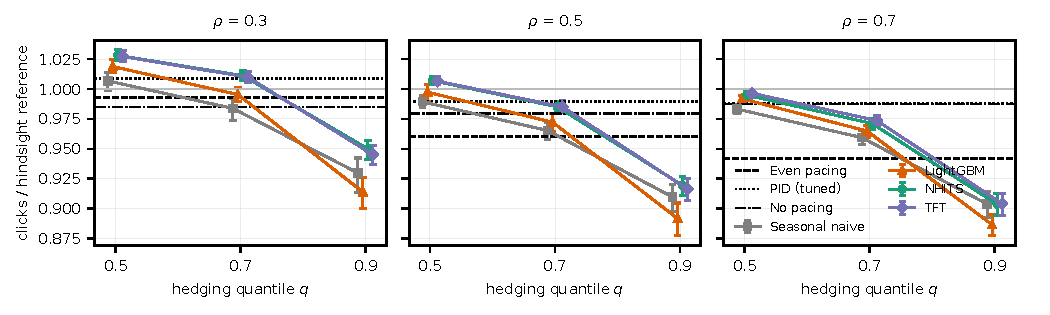
\includegraphics[width=\textwidth]{fig_hedging.pdf}
  \Description{Three budget panels show declining click ratios as the planning
  quantile rises. Horizontal lines mark the forecast-free policies.}
  \caption{Click ratio versus planning quantile (95\% campaign-bootstrap CIs). Horizontal lines are forecast-free policies.}
  \label{fig:hedging}
\end{figure*}
Clicks fall as $q$ rises from 0.5 to 0.9 in all \res{hedge-mono} of
\res{hedge-mono-total} forecaster-and-budget combinations, costing
\res{hedge-cost-min}--\res{hedge-cost-max} points (Figure~\ref{fig:hedging}).
Upper plans cut early depletion to \res{hedge-early-min}--\res{hedge-early-max}\%
of episodes, but budget utilization falls to
\res{hedge-bur-min}--\res{hedge-bur-max}\%. Summed hourly 90\% quantiles
over-cover the remaining-day total (\res{hc-cov90-min}--\res{hc-cov90-max}\%
coverage). Rescaling the median plan by factors calibrated on earlier test
days recovers \res{ch-rec-rho0.3}\%, \res{ch-rec-rho0.5}\% and
\res{ch-rec-rho0.7}\% of TFT's $q=0.9$ loss, which falls short of the protocol's
one-third threshold. The replay rewards clicks and barely penalizes early
exhaustion, so this cost partly reflects the objective.

\subsection{Robustness checks}
\textbf{Other reactive rules.} A tuned dual-gradient throttle
\cite{balseiro2019learning} does not beat PID, and TFT leads its corrected
variant by \res{dg-tft-profn-min}--\res{dg-tft-profn-max} points.
\textbf{Feedback.} Adding PID feedback to the forecast rate, with gains tuned
on seasonal naive, does not improve TFT at two of three budgets, and TFT then
no longer clearly beats scaled naive with feedback. \textbf{A synthetic
world.} In generated worlds with planted rhythms, replaying the previous week
gains \wres{replay-gain-min}--\wres{replay-gain-max} points over reactive
control, and a perfect daily total adds only \wres{total-min}--\wres{total-max}.
\textbf{iPinYou.} On \res{ipy-advertisers} advertisers and
\res{ipy-episodes} test episodes, the naive-over-even differences have CIs
that include zero, and the Criteo ordering holds at \res{ipy-consistent} of 3 budget
levels. No neural models were tested there.

% ------------------------------------------------------------------
\section{Discussion and Conclusion}

On Criteo, all five tested neural predictors capture more clicks than seasonal
naive under the same throttle, mainly by spending more of the budget with
similar clicks per unit of spend. In TFT's swap experiment most of the gain
comes from the daily total. A single validation-chosen scale recovers much of
it at the loose budget but less than half at the tight one, and a gain
remains at matched aggregate spend whose cause is unresolved. Upper-quantile
plans leave budget unspent in this click-focused replay, and calibration
recovers only part of that loss.

\textbf{Limitations.} The test period is \res{cfg-test-days} days of one
dataset. Intervals condition on saved models and exclude seed uncertainty. The
replay uses won impressions and transformed prices, without price responses or
an explicit cost of early exhaustion. Day boundaries are relative to the
dataset start. The main design was informed by a full-data profile, and the
follow-up analyses reused the same test days after the main results were
known. Tuning used only \res{cfg-val-days} validation days. The iPinYou check
is small and tests no neural models. Next steps are seed-aware inference,
longer out-of-time evaluation on other real logs, and a simulator with price
responses and delivery constraints. Code, protocol and results will be
released.

\section*{Use of Generative AI Tools}
Claude (Anthropic) and an OpenAI assistant helped with code, experiments,
writing and draft review. Numerical results come from the accompanying code.
Model feedback is not human peer review. The author is responsible for the
content.

\bibliographystyle{ACM-Reference-Format}
\bibliography{references}

\end{document}
